%\documentclass{hotnets22}
% \documentclass[sigconf,10pt]{acmart}
\documentclass[letterpaper,twocolumn,10pt]{article}
\usepackage{usenix-2020-09}
\usepackage{amsmath}

\usepackage{times}  
\usepackage{hyperref}
\usepackage{subfig}
\usepackage{tikz}
\usetikzlibrary{math}
\usepackage{pgfplots}
\usepackage{pgfplotstable}

\hypersetup{pdfstartview=FitH,pdfpagelayout=SinglePage}

\setlength\paperheight {11in}
\setlength\paperwidth {8.5in}
\setlength{\textwidth}{7in}
\setlength{\textheight}{9.25in}
\setlength{\oddsidemargin}{-.25in}
\setlength{\evensidemargin}{-.25in}

\newcommand{\rg}[1]{\textcolor{blue}{(\textbf{GR:} #1)}}

% TODO: remove for the CR!
% \pagestyle{plain}
% \settopmatter{printfolios=true}

\begin{document}

% \conferenceinfo{HotNets 2022} {}
% \CopyrightYear{2022}
% \crdata{X}
% \date{}

% \pgfplotsset{
%     cont/.style={
%         cont/.style={red},
%     },
%     dshd/.style={
%         dshd/.style={},
%     },
% }

%%%%%%%%%%%% THIS IS WHERE WE PUT IN THE TITLE AND AUTHORS %%%%%%%%%%%%

%\title{Network Goodput beyond Amdahl’s Law\\with Parallel Self-adjusting Data Structures}
% \title{Beyond Amdahl's Law: Superlinear Scaling with Self-adjusting Distributed Systems}
\title{Beyond Amdahl's Law: Achieving Superlinear Scaling with Self-adjusting Distributed Systems}

\author{Paper \#??} %, 6 + 1 pages}

\maketitle

\tableofcontents

%%%%%%%%%%%%% ABSTRACT GOES HERE %%%%%%%%%%%%%%
\begin{abstract}
  With the end of Moore's law and the quick transition to hyperscale cloud platforms, computing power in modern computing systems increasingly comes in the form of parallel processing resources.  A major obstacle faced by network engineers is how to harness this increasingly parallel computing power, given that Amdahl's law predicts sublinear scaling and diminishing returns for massive-scale parallelization.  In this paper, we propose the combination of \emph{locality-boosting load balancing} and \emph{self-adjusting data structures} to sidestep Amdahl's law and achieve superlinear initial scaling for typical massively parallel networking workloads. We demonstrate quadratic scale-up on several artificial models and a multi-threaded packet classifier, and, strikingly, we find that parallelization yields linear speedup even if we keep the total available computing power constant. We argue that, in light of our results, it is time to revisit the applicability of Amdahl's law to future massive-scale networked systems.
\end{abstract}

\section{Introduction}\label{sec:introduction}

\section{Background}\label{sec:background}

\subsection{The Load Balancer Pattern}
\label{sec:lb-pattern}

A common architectural design pattern for scaling distributed applications to parallel computing resources, such as CPU cores, containers\slash pods\slash VMs, servers, or entire computer clusters, is the \emph{load balancer model} \cite{10.5555/3235491}.  Here, a load balancer dispatches requests across a fleet of parallel workers using a simple policy (random, round robin, sticky sessions, etc.), which then process the requests independently and return the results back to the clients.

As the simplest choice for optimizing resource use, maximizing throughput, and minimizing response time, the load balancer pattern is ubiquitous in networking. Multicore \emph{OS network stacks} \cite{211263, 10.1145/3359989.3365412, 10.1145/3452296.3472914} leverage the NIC to dispatch packets across the CPU cores. In order to avoid packet reordering and improve CPU cache performance, load balancing typically occurs by the NIC computing a hash over the packet header, e.g., the IP 5-tuple (RSS, RPS, etc.).  In the context of \emph{web applications}, HTTP load balancers \cite{194966, 211279, 9552525} distribute requests across a swarm of backend servers by hashing over the source IP address (``sticky-sessions''). This way, requests from the same client will hit the same backend server, improving request locality and hence, performance. In massive-scale \emph{key-value stores} \cite{ghigoff2021bmc}, the key-space is hashed into multiple shards (partitions) and each shard is assigned to a separate server. Then, queries are distributed over the shards by hashing the requested key. From distributed cache servers to microservice applications, the load balancing pattern is everywhere in modern large-scale networked systems.

\begin{figure}[t]
  \centering
  % \includegraphics[width=0.8\linewidth]{fig/usl.png}
  \begin{small}
  \begin{small}
  \begin{tikzpicture}[remember picture]
    \begin{axis}[
      width=250pt,
      height=170pt,
      xlabel={\#threads},
      ylabel={Speedup},
      xlabel near ticks,
      ylabel near ticks,
      xmin=1,
      xmax=25,
      ymin=1,
      ymax=90,
      xtick={1,5,10,15,20,24},
      legend style = {
        anchor = north west,
        at = {(rel axis cs:0.01,0.98)},
        font=\scriptsize,
        % draw = none,
      },
      no markers
      ]
      % use TeX as calculator:
      \addplot[domain=1:25,black,densely dotted]{x};
      \addlegendentry{Linear scaling}

      \addplot[domain=1:25,black,densely dashed]{1/(0.01 + (1-0.01)/x)};
      \addlegendentry{Amdahl's law}

      \addplot[domain=1:25,black,solid]{1/(0.01 + (1-0.01)/x^2)};
      \addlegendentry{Proposed scaling law}

      \coordinate (insetPosition) at (rel axis cs:.97,0.25);
      % \addplot[domain=0:15,black,loosely dashed]{1/(0.4 + (1-0.4)/x)};
      % \addlegendentry{Amdahl's law ($\delta=0.4$)}

      % \addplot[domain=0:15,black,loosely dotted]{1/(0.4 + (1-0.4)/x^2)};
      % \addlegendentry{Proposed scaling law for MTF ($\delta=0.4$)}
    \end{axis}
    \begin{axis}[
      at={(insetPosition)},
      anchor={outer south east},
      width=105pt,
      height=85pt,
      tiny,
      % xlabel={\#cores},
      % ylabel={Speedup},
      xmin=1,
      xmax=450,
      ymin=0,
      ymax=110,
      % ytick={1,2,3,4,5},
      no markers]
      \addplot[domain=1:500,black,densely dotted]{x};
      \addplot[domain=1:500,black,densely dashed]{1/(0.01 + (1-0.01)/x)};
      \addplot[domain=1:500,black,solid]{1/(0.01 + (1-0.01)/x^2)};
    \end{axis}
  \end{tikzpicture}
\end{small}

%%% Local Variables:
%%% mode: latex
%%% TeX-master: "../distributed_mrf.tex"
%%% End:

\end{small}
  \caption{Linear scaling, Amdahl's law and the proposed scaling law ($s=0.01$). The inset shows the asymptotics.}
  \label{fig:amdahl}
\end{figure}

But do load balancers really scale? In this paper, we argue that \emph{they may scale even better than you might have expected}: we show that, compared a typical concurrent system for which Amdahl's law (\S\ref{sec:amdahl-law}) predicts strictly sublinear scaling and diminishing returns for parallelization (see the inset in Fig.~\ref{fig:amdahl}), the combination of \emph{locality boosting load balancing} (\S\ref{sec:scal-distr-cach}) and worker threads implemented using \emph{self-adjusting data structures}  (\S\ref{sec:parallel-move-front}) unlocks faster-than-linear initial scaling (see the proposed scaling law in Fig.~\ref{fig:amdahl} and a discussion in \S\ref{sec:discussion}). What is more, we are able to reproduce the superlinear scaling trend in a real-life application: we sketch a self-adjusting packet classifier that achieves $600\times$ speedup~(!) on $60$ parallel threads, which is $10\times$ of what is predicted by Amdahl's law (\S\ref{sec:packet-classifier}).

\subsection{Amdahl's Law}
\label{sec:amdahl-law}

A cornerstone result in parallel computing, Amdahl's law \cite{10.1145/1465482.1465560} establishes a firm limit on the performance gain obtainable by distributing a computation task over multiple processors. Given a partially parallel program, denote the fraction of execution time spent % by a single-threaded execution
% by the processor 
in the serial part of the code by $s$, and the parallel fraction by $(1-s)$. Here, some code is ``serial'' if it cannot benefit from the improvement of the computing resources, like single-threaded code, critical sections guarded by exclusion locks, etc. Denote by $T(k)$ the runtime (in seconds) of the program when executed on $k$ processors, and let $S(k)=\frac{T(1)}{T(k)}$ denote the  performance improvement relative to a single-threaded execution (i.e., the \emph{speedup}). Then, the following relation holds:
\begin{equation}\label{eq:amdahl}
S(k) = \frac{T(1)}{T(k)} = \frac{1}{s + \frac{1-s}{k}} \enspace .
\end{equation}

Here, the term $\frac{1-s}{k}$ establishes that the perfectly parallel part of the program executes $k$ times faster on $k$ processors than on a single core. By Amdahl's law, (1) no code can scale faster than linear (i.e., $\frac{d S(k)}{d k} \le 1$, with equality exactly when $s=0$), (2) throwing additional processors on a computation task yields diminishing returns ($\frac{d S(k)}{d k}$ is decreasing in $k$) and (3) the asymptotics is limited by the serial part only ($\lim_{k\to \infty}S(k) = \frac1{s}$). Despite often being misused \cite{10.5555/775339.775386}, debated \cite{10.1145/42411.42415} and extended \cite{4563876, 6280307,1580395,406581,6163449}, Amdahl's law has remained one of the most useful tools in the system engineering toolbox to today \cite{10.5555/1951599}. %A sample plot is given in Fig.~\ref{fig:amdahl}. 

It is then simple to apply Amdahl's law in the load-balancer architecture: the load balancer itself corresponds to the serial workload and the workers constitute the parallel part. Since networking workloads are typically massively parallel (so $s \ll 1$) we expect close-to-linear scaling, at least in the initial regime of the scalability plot (i.e., for small values of $k$). A simple example, however, casts a completely different picture.

% \begin{figure}
%   \centering
%   \begin{tiny}
% \begin{verbatim}
%                                      +--------+
%                               +----->|Thread 1|
%                               |      +--------+
%                               |
%                               |      +--------+
% +------+    +-------------+   +----->|Thread 2
% |Source|----|Load-balancer|---+      +--------+
% +------+    +-------------+   |          .
%                               |          .
%                               |          .
%                               |      +--------+
%                               +----->|Thread k|
%                                      +--------+
% (placeholder)
% \end{verbatim}
%   \end{tiny}
%   \caption{A typical distributed computing architecture.}
%   \label{fig:model}
% \end{figure}

Fig.~\ref{fig:multicore-cache} plots a scalability benchmark obtained on a makeshift distributed caching system, implemented in a couple of hundred lines of Go and deployed to a CoTS blade server with a 24-core Intel CPU. % (see [GITHUB LINK WILL BE REVEALED IN THE FINAL VERSION])
Here, 1000 items are stored in $k$ independent least-recently-used (LRU) caches, executing in lightweight parallel execution threads (``goroutines''). A simple serial load balancer, first using round robin and then with hashing over the request id, spreads requests across the parallel caches. Requests are distributed uniformly across the 1000 items, which is a trivial worst-case input for LRU caches.

\begin{figure}
  \centering
  % \subfloat[][multicore]{
  \pgfplotsset{
  RatePlot/.style = {
    tick pos = left,
    xtick align=outside,
    ytick align=outside,
    xlabel near ticks,
    ylabel near ticks,
    width=.4\textwidth,
    height=.3\textwidth,
    legend pos = north west,
    legend cell align=left,
    ylabel = {Throughput [Mpps]},
    xlabel = {number of CPU cores},
    xmin=1, xmax=32,
    ymin=0,
  },
  SpeedupPlot/.style = {
    RatePlot,
    ylabel={Speedup},
  },
  ClassBenchGroupPlot/.style = {
    group/group size = 1 by 2,
    group/horizontal sep = 0pt,
    group/vertical sep = 28pt,
  },
  ClassBenchRatePlot/.style = {
    RatePlot
  },
  ClassBenchSpeedupPlot/.style = {
    SpeedupPlot,
  }
}

%%% Local Variables:
%%% mode: latex
%%% TeX-master: "../distributed_mrf.tex"
%%% End:

%
\begin{small}
  % \tikzmath
  % {
  %   function est(\x)
  %   {
  %     if (\x < 10) then
  %     {
  %       return 0.1+0.9*(0.1*\x +(1-0.1*\x)*10)/\x;
  %     } else {
  %       return 0.1 + 0.9//\x;
  %     };
  %   };
  %   \a = est(4);
  %   \b = est(14);
  % }
  \begin{tikzpicture}
    \begin{axis}[
      width=165pt,
      height=120pt,
      xlabel={\#CPU cores},
      x label style={at={(0.5,0.04)}},
      ylabel={Speedup},
      % xlabel near ticks,
      % ylabel near ticks,
      y label style={at={(0.1,0.5)}},
      xmin=1,
      xmax=35,
      ymin=0,
      xtick={1,10,20, 30},
      % ymax=10,
      legend style = {
        anchor = north west,
        at = {(0.01, 1.01)},
        font=\scriptsize,
        % draw = none,
      },
      % no markers
      ]
      \addplot[SelfAdjustingSimMark,mark size=2pt] table[x=thread,y=speedup,each nth point={3}]{fig/cache/uniform-50k-2/mcore_cache_modulo_uniform.txt};
      % \addlegendentry{Local LB}
      \addplot[SelfAdjustingSimMark,mark=pentagon*,mark size=3pt,each nth point={3}] table[x=thread,y=speedup,each nth point={2}]{fig/cache/uniform-50k-2/mcore_cache_roundrobin_uniform.txt};
      % \addlegendentry{Non-local LB}
      % \addplot[domain=1:25,black,dashed]{x};
      % \addlegendentry{Linear scaling}
      % \addplot[domain=1:25,black,densely dotted]{1/(0.03+0.97/x)};
      % \addlegendentry{Amdahl's law}
      % \addplot[domain=0:25,black,densely dotted]{est(1.0)/est(x)};
      % \node at (100,100) {\a\b};
      % \addlegendentry{T}
      % \addplot[black,mark=o] table[x=thread,y=rate] {fig/cache/uniform-50k/multicore_cache_roundrobin_uniform.txt};
      % \addlegendentry{Round robin lb}
      % \addplot[black,mark=square] table[x=thread,y=rate] {fig/cache/uniform-50k/multicore_scache_roundrobin_uniform.txt};
      % \addlegendentry{staticcache / roundrobin}
    \end{axis}
  \end{tikzpicture}
\end{small}

%%% Local Variables:
%%% mode: latex
%%% TeX-master: "../../../distributed_mrf"
%%% End:

  % \label{fig:multicore-cache-uniform-10}
  % }
  % \subfloat[][multicore2]{\input{fig/cache/uniform-3000/multicore_cache_roundrobin.tex}\label{fig:multicore-cache-uniform-10-2}}
  % \subfloat[][singlecore]{\input{fig/bsinglecore_tree.tex}\label{fig:singlecore-list-uniform-10}}
  \caption{Distributed cache speedup over uniformly distributed requests, $m=1000$}
  \label{fig:multicore-cache}
\end{figure}

Clearly, distributed caching adheres to Amdahl's law, at least as long as the load balancing policy is round robin. But when load balancing uses the id hash we see something unexpected: we observe a rapid superlinear scaling, with $50\times$ speedup at 20 cores compared to the single-threaded case. This is $2.5\times$ faster than predicted by Amdahl's law.

What is going on here? How can such a simple distributed application violate Amdahl's law (if at all)? The rest of this paper is devoted to an attempt to answer these questions. % We argue that the load balancer % distributed system
% pattern, with a combination of a \emph{locality boosting load balancing} (like, e.g., id hashing above) and worker threads implemented using \emph{self-adjusting data structures}, has the potential to unlock faster-than-linear initial scaling for massive-scale networked applications. We also derive the corresponding scaling law for some select use cases; see Fig.~\ref{fig:amdahl} for an example.

% \subsection{Extensions to Amdahl's Law}
% \label{sec:extended-amdahl-law}

\section{Motivation: Distributed Caches}
\label{sec:motivation}

ARGUE THAT DISTRIBUTED CACHES HAVE BEEN DELIVERING SUPERLINEAR FOR AGES (ref papers!)

Caches are really the simplest mechanism that can ``self-adjust'' to the input thrown at them (self-adjustments will come up below frequently!): a cache will keep recent, or frequently-used, data items in fast storage, where access is much more efficient than from normal storage, in order to improve lookup time for future requests. Today we get efficient caches built into all modern CPUs, but many networking applications explicitly contain a fast-path\slash cache component; e.g., distributed caches (e.g., \texttt{memcached}) used as a fast frontend for a ``slow'' web service or relational database, popular keys offloaded to the OS kernel for fast access into key-value stores \cite{179747, ghigoff2021bmc}, FIB caches that maintain the most frequent IP routes in a fast-path cache to sidestep slowish longest prefix matching \cite{rottenstreich2016optimal}, hierarchical flow-caches that serve as a fast-path in programmable software switches \cite{188960}, etc. It is then somewhat surprising that such simple distributed LRU caches alone, paired with a proper load balancing policy like id-hashing, can already provide superlinear (initial) scaling beyond what's predicted by Amdahl's law\footnote{We theoretize that, perhaps without knowing, the prospect of superlinear scaling is \emph{exactly} the reason for the ubiquitous use of caches in networking.} (recall Fig.~\ref{fig:multicore-cache}).

Clearly, cache performance benefits if the instances tend to process requests to the same or ``similar'' items. This is because caches can effectively ``self-adjust'' to the input: frequently accessed items will be migrated to fast memory where they can be served more efficiently, and the overall lookup time, averaged over all cache instances and all requests, will decrease. The load balancer policy will then be responsible for \emph{boosting the locality of reference} in the input processed by each cache instance. For instance, when the NIC dispatches ingress packets based on the IP 5-tuple hash it effectively partitions the active flow set across the cores, so that each of the $k$ worker threads will encounter only $\frac1{k}$ fraction of all active flows processed by the system (see Fig.~\ref{fig:locality-boosting-lb}). Sharded key-value stores carefully organize shards so that each server will process only $\frac1{k}$ fraction of the total key space.  This is in contrast to round-robin or random load-balancing, which exports the exact same locality in the system input to the workers.

\begin{figure}[t]
  \centering
  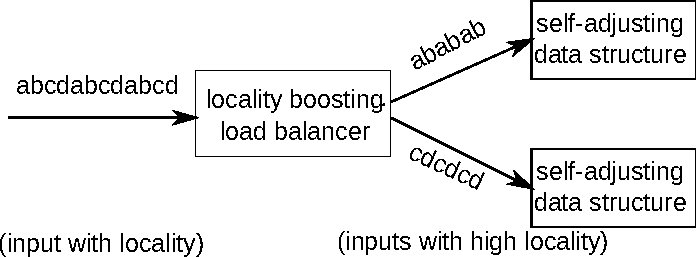
\includegraphics[width=.85\linewidth]{fig/schema.pdf}
  \caption{A locality boosting load balancer partitions the input sequence of a given locality into
    subsequences with higher locality. Self-adjusting data structures perform better on inputs with
    higher locality.}
  \label{fig:locality-boosting-lb}
\end{figure}

We call a request dispatching strategy that improves the temporal and\slash or spatial locality as experienced by the worker threads as a \emph{locality boosting load balancing policy}, and we identify such locality boosting load balancers as the first key ingredient in the superlinear scaling of distributed systems.

A quick back-of-an-envelope analysis will help quantify the effect of locality boosting in distributed caches. Suppose a source emits uniformly distributed random requests for $m$ items and the load balancer dispatches requests by hashing on the request id. This effectively partitions the requests into $k$ random buckets, so that each cache instance will experience uniformly distributed requests for only $\frac{m}{k}$ items. If the cache hit rate for a single LRU cache instance processing $m$ requests is $\delta$, then our locality boosting load balancer will improve the cache hit rate to $k\delta$ for $k$ threads ($k\delta \le 1$). This puts the lookup time of the system of $k$ parallel caches to
\begin{align}\label{eq:dist-cache}
  T_c(k) = \begin{cases} s + \frac{1-s}{k}(k\delta + (1-k\delta)\rho) & \text{if } k\delta \le 1\\s + \frac{(1-s)}{k} & \text{otherwise}\end{cases} \enspace ,
\end{align}
where $\rho$ is the penalty for a cache miss event.

The speedup $S_c(k)=\frac{T_c(1)}{T_c(k)}$ is depicted in Fig.\ref{fig:dcache-analysis}. The lower envelope of the scaling profile is given by Amdahl's law for the system with round-robin load-balancing ($\frac{T_c(1)}{s + \frac{1-s}{k}(\delta + (1-\delta)\rho)}$), from which the profile progresses over a superlinear curve to an elevated Amdahl's law profile, representative of a system where \emph{all} requests are served from fast memory ($\frac{T_c(1)}{s + \frac{1-s}{k}}$).

\begin{figure}[t]
  \centering
  \begin{small}
    \begin{small}
  \tikzmath
  {
    function lookup(\x)
    {
      if (\x < 10) then
      {
        return 0.1+0.9*(0.1*\x +(1-0.1*\x)*10)/\x;
      } else {
        return 0.1 + 0.9/\x;
      };
    };
    function dcache(\x)
    {
      return lookup(1.0)/lookup(\x);
    };
    function rrcache(\x)
    {
      return lookup(1.0)/(0.1+0.9*(0.1 +(1-0.1)*10)/\x);
    };
    function pcache(\x)
    {
      return lookup(1.0)/(0.1+0.9/\x);
    };
    \a = dcache(1);
    \b = lookup(1.0);
  }
  \begin{tikzpicture}
    \begin{axis}[
      width=250pt,
      height=170pt,
      xlabel={\#threads},
      ylabel={Speedup},
      xlabel near ticks,
      ylabel near ticks,
      xmin=0,
      xmax=20,
      ymin=0,
      ymax=67,
      xtick={1,5,10,15,20},
      legend style = {
        anchor = north west,
        at = {(0.01, 1.01)},
        font=\scriptsize,
        % draw = none,
      },
      % no markers
      ]
      \addplot[domain=0:25,black,solid]{dcache(x)};
      \addlegendentry{Hash-based load balancing}
      \addplot[domain=0:25,black,densely dotted]{rrcache(x)};
      \addlegendentry{Random load balancing}
      \addplot[domain=0:25,black,densely dashed]{pcache(x)};
      \addlegendentry{All requests hit the cache}
      % \node at (25,25) {\a, \b};
    \end{axis}
  \end{tikzpicture}
\end{small}

%%% Local Variables:
%%% mode: latex
%%% TeX-master: "../distributed_mrf"
%%% End:

\end{small}
\caption{Scaling laws for distributed caching: hash-based load balancing, lower envelope (round robin load balancing) and upper envelope (perfect cache hit rate with $k$ caches). Parameters: $s=0.1$, $\delta=0.1$ and $\rho=10$.}
  \label{fig:dcache-analysis}
\end{figure}

One could convincingly argue that this is cheating, and a misuse of Amdahl's law \cite{10.5555/775339.775386}: by dropping additional cache instances to the system we effectively multiply the available fast memory, and this will trivially lead to faster access times. For multicore CPU systems this argumentation would clearly pass muster: since L2/L3 caches are typically shared across cores (but L1 caches are not!), so new threads will not improve performance, only worsen CPU cache contention \cite{manousis-sigcomm20, 211291}. We observe, however, that increasing the available fast memory is \emph{exactly the idea} in many common use cases, like adding \texttt{memcached} instances to a storage network or additional Redis replicas to sharded database cache.\footnote{Whether the superlinear scaling predicted by the model manifests itself with such real-life use cases is open for future research; we theoretize (without experimental evidence) that the answer is affirmative.}

%PROBLEM STATEMENT

But more importantly, we argue that distributed caching is just one application, and not necessarily the most illustrative one, of a more general scheme, namely that locality boosting load balancing and self-adjusting data structures \emph{combined} can effectively achieve superlinear scaling in many use cases.

\section{Distributed Self-adjusting Algorithms}
\label{sec:parallel-move-front}

In the previous section we identified locality boosting load balancing as a key for superlinear scaling. Indeed, hashing essentially partitions the id space across the threads, which now experience only a fraction of the working set size, leading to faster lookups. Of course, this holds only as far as the worker threads, and in particular the algorithms running inside the threads, can take advantage of the improved locality of reference. LRU caches are perfectly positioned for this, by adjusting the set of items kept in fast memory to the item popularity. At the same time, caches fundamentally rely on fast memory, and in certain use cases (like multicore CPUs) adding further fast memory to the system is not possible.

In general, caches are just one example of the broader category of \emph{self-adjusting data structures}. A self-adjusting data structure can rearrange itself as queries are committed to it, in order to improve efficiency on future requests. In this context, a ``static cache'', which keeps an arbitrary set of items in fast memory without cache eviction, is not self-adjusting, while an LRU\slash LFU cache is. As another example, an AVL tree is not self-adjusting in that it can rearrange only with respect to the items \emph{stored} in it but not with respect to the queries \emph{committed} to it, whereas a splay tree is self-adjusting in that it can dynamically move popular items towards the root of tree, improving future access to the same or similar items \cite{SleatorT85Splay, BoseDL08, Avin0020}. Self-adjusting data structures are widely used in algorithms and computer systems, e.g., in computing point maxima and convex hulls~\cite{BentleyCL93}, organizing lists of identifiers in program compilation and interpretation~\cite{HesterH85}, detecting collisions in hash tables~\cite{HesterH85}, or compressing arbitrary input~\cite{BentleySTW86}. And indeed, every cache management scheme can be viewed as a self-adjusting data structure as well % , in that every algorithm for list reorganization gives rise to a different cache management algorithm~
\cite{SleatorT85}.  % Further self-adjusting data structures include splay trees~\cite{SleatorT85Splay}, self-adjusting skip lists~\cite{BoseDL08}, push-down trees~\cite{Avin0020}, or self-adjusting trees for storing geometric data \cite{ParkM12}.

\begin{figure}[t]
  \centering
  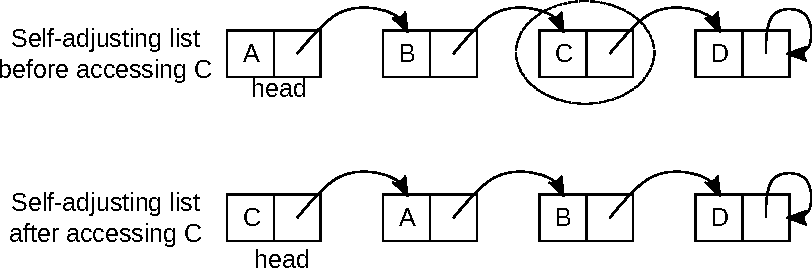
\includegraphics[width=.85\linewidth]{fig/mtf.pdf}
  \caption{A self-adjusting list containing nodes A,B,C and D serves the request to C and moves C to the front of the list to speed up future accesses to C.}
  \label{fig:mtf-example}
\end{figure}

\begin{figure*}[t]
    \centering
    \subfloat[][multicore]{\begin{small}
  \begin{tikzpicture}
    \begin{axis}[
      width=165pt,
      height=322pt,
      xlabel={number of CPU cores},
      x label style={at={(0.5,0.01)}},      
      ylabel={Speedup},
      y label style={at={(0.05,0.5)}},      
      xmin=1,
      xmax=48,
      xtick={1,12,24,36,48},
      ymin=0,
      ymax=3300,
      legend style = {
        anchor = north west,
        at = {(0.01, 1.01)},
        font=\tiny,
        % draw = none,
      },
      % scaled y ticks=false
      % no markers
      ]
      % use TeX as calculator:
      \addplot[black,mark=*] table[x=thread,y=speedup,] {fig/list/uniform-100k/multicore_mtf_modulo_uniform.txt};
      % \addlegendentry{Move-to-front/Local LB}
      \addplot[black,mark=+] table[x=thread,y=speedup,each nth point={3}] {fig/list/uniform-100k/multicore_linkedlist_modulo_uniform.txt};
      % \addlegendentry{Linked-list/Local LB}
      \addplot[black,mark=o] table[x=thread,y=speedup,each nth point={3}] {fig/list/uniform-100k/multicore_mtf_roundrobin_uniform.txt};
      % \addlegendentry{Move-to-front/Non-local LB}
      \addplot[black,mark=square] table[x=thread,y=speedup,each nth point={3}] {fig/list/uniform-100k/multicore_linkedlist_roundrobin_uniform.txt};
      % \addlegendentry{Linked-list/Non-local LB}
    \end{axis}
  \end{tikzpicture}
\end{small}

%%% Local Variables:
%%% mode: latex
%%% TeX-master: "../../../distributed_mrf"
%%% End:
\label{fig:multicore-list-uniform-10}}
    \hfill%
    \subfloat[][singlecore]{\begin{small}
  \begin{tikzpicture}
    \begin{axis}[
      width=250pt,
      height=170pt,
      xlabel={\#thread},
      ylabel={Goodput [million req/sec]},
      xlabel near ticks,
      ylabel near ticks,
      xmin=1,
      xmax=26,
      ymin=0,
      % ymax=10,
      legend style = {
        anchor = north west,
        at = {(0.01, 1.01)},
        font=\scriptsize,
        % draw = none,
      },
      % no markers
      ]
      \addplot[black,mark=*] table[
      x=thread,
      y expr=\thisrowno{4}/1000000
      ]{fig/list/uniform-10/singlecore_mtf_modulo_uniform.txt};
      \addlegendentry{MTF w/ hash-based lb}
      \addplot[black,mark=+] table[
      x=thread,
      y expr=\thisrowno{4}/1000000
      ]{fig/list/uniform-10/singlecore_linkedlist_modulo_uniform.txt};
      \addlegendentry{Static list w/ hash-based lb}
      \addplot[black,mark=o] table[
      x=thread,
      y expr=\thisrowno{4}/1000000
      ]{fig/list/uniform-10/singlecore_mtf_roundrobin_uniform.txt};
      \addlegendentry{MTF w/ round robin lb}
      \addplot[black,mark=square] table[
      x=thread,
      y expr=\thisrowno{4}/1000000
      ]{fig/list/uniform-10/singlecore_linkedlist_roundrobin_uniform.txt};
      \addlegendentry{Static list w/ round robin lb}
    \end{axis}
  \end{tikzpicture}
\end{small}

%%% Local Variables:
%%% mode: latex
%%% TeX-master: "../../../hotnets22"
%%% End:
\label{fig:singlecore-list-uniform-10}}
    \caption{Linked list lookup scaling over uniformly distributed requests, $m=10000$: (a) no upper bound on the number of CPU cores available to the system, (b) limiting the total system load at $110$\%.}
  \label{fig:multicore-list}
\end{figure*}

\begin{figure*}[t]
  \centering
  \subfloat[][multicore]{\begin{small}
  \begin{tikzpicture}
    \begin{axis}[
      width=165pt,
      height=322pt,
      xlabel={number of CPU cores},
      x label style={at={(0.5,0.01)}},      
      ylabel={Speedup},
      y label style={at={(0.05,0.5)}},      
      xmin=1,
      xmax=48,
      xtick={1,12,24,36,48},
      ymin=0,
      ymax=3300,
      legend style = {
        anchor = north west,
        at = {(0.01, 1.01)},
        font=\tiny,
        % draw = none,
      },
      % scaled y ticks=false
      % no markers
      ]
      % use TeX as calculator:
      \addplot[black,mark=*] table[x=thread,y=speedup,] {fig/list/uniform-100k/multicore_mtf_modulo_uniform.txt};
      % \addlegendentry{Move-to-front/Local LB}
      \addplot[black,mark=+] table[x=thread,y=speedup,each nth point={3}] {fig/list/uniform-100k/multicore_linkedlist_modulo_uniform.txt};
      % \addlegendentry{Linked-list/Local LB}
      \addplot[black,mark=o] table[x=thread,y=speedup,each nth point={3}] {fig/list/uniform-100k/multicore_mtf_roundrobin_uniform.txt};
      % \addlegendentry{Move-to-front/Non-local LB}
      \addplot[black,mark=square] table[x=thread,y=speedup,each nth point={3}] {fig/list/uniform-100k/multicore_linkedlist_roundrobin_uniform.txt};
      % \addlegendentry{Linked-list/Non-local LB}
    \end{axis}
  \end{tikzpicture}
\end{small}

%%% Local Variables:
%%% mode: latex
%%% TeX-master: "../../../distributed_mrf"
%%% End:
\label{fig:multicore-list-poisson-300}}
    \hfill%
  \subfloat[][singlecore]{\begin{small}
  \begin{tikzpicture}
    \begin{axis}[
      width=250pt,
      height=170pt,
      xlabel={\#thread},
      ylabel={Goodput [million req/sec]},
      xlabel near ticks,
      ylabel near ticks,
      xmin=1,
      xmax=26,
      ymin=0,
      % ymax=10,
      legend style = {
        anchor = north west,
        at = {(0.01, 1.01)},
        font=\scriptsize,
        % draw = none,
      },
      % no markers
      ]
      \addplot[black,mark=*] table[
      x=thread,
      y expr=\thisrowno{4}/1000000
      ]{fig/list/uniform-10/singlecore_mtf_modulo_uniform.txt};
      \addlegendentry{MTF w/ hash-based lb}
      \addplot[black,mark=+] table[
      x=thread,
      y expr=\thisrowno{4}/1000000
      ]{fig/list/uniform-10/singlecore_linkedlist_modulo_uniform.txt};
      \addlegendentry{Static list w/ hash-based lb}
      \addplot[black,mark=o] table[
      x=thread,
      y expr=\thisrowno{4}/1000000
      ]{fig/list/uniform-10/singlecore_mtf_roundrobin_uniform.txt};
      \addlegendentry{MTF w/ round robin lb}
      \addplot[black,mark=square] table[
      x=thread,
      y expr=\thisrowno{4}/1000000
      ]{fig/list/uniform-10/singlecore_linkedlist_roundrobin_uniform.txt};
      \addlegendentry{Static list w/ round robin lb}
    \end{axis}
  \end{tikzpicture}
\end{small}

%%% Local Variables:
%%% mode: latex
%%% TeX-master: "../../../hotnets22"
%%% End:
\label{fig:singlecore-list-poisson-300}}
  \caption{Linked list lookup scaling over a Poisson request distribution, $m=30000$, $\lambda=2$: (a) no upper bound on the number of CPU cores available to the system, (b) limiting the total system load at $110$\%.}
  \label{fig:multicore-list-poisson}
\end{figure*}

Perhaps the best-known general self-adjusting data structure is the \emph{move-to-front list}. Suppose we wish to store a list of $m$ items in a way so that reordering, insertion and deletion is fast, while lookup is also ``reasonably'' efficient. A straightforward choice is a (singly) linked list. Here, the cost of accessing an item at position $i$ is exactly $i$. Then, a static linked list can easily be upgraded to a self-adjusting list using the move-to-front (MTF) heuristics: after accessing an item we move it to the front of the list (see Fig.~\ref{fig:mtf-example}). As such a reordering is supposed to be ``cheap'', MTF generally improves lookup time for future requests of the same item at minimal cost.

% <PLACEHOLDER FOR MACIEK: discuss MTF lists without going into details, give examples with figs, and applications. Remember, we want to popularize the idea across the systems community, so be as gentle to practitioners as possible.>

Classic applications of MTF lists are information retrieval systems, compression~\cite{BentleySTW86}, etc. In network applications, however, where static linked lists enjoy wide applicability, e.g., for rule matching in OpenFlow and P4 reference software switches, packet classification in the Linux OS network stack (\texttt{iptables}), etc., so far we haven't seen many uses of the self-adjusting version, i.e., MTF lists. We imagine potential applications in packet classification (see later in \S\ref{sec:packet-classifier}), flow table lookup, evaluating rules in an intrusion detection system, etc.; in general, all networking use cases are relevant where ``matching'' a request against a list item is costly and the items do not lend themselves readily to be arranged into a fast lookup structure (like a search tree).

It is now straightforward to modify our benchmark to store items in MTF lists instead of LRU caches. Fig.~\ref{fig:multicore-list} shows the experimental results for uniformly distributed requests, and Fig.~\ref{fig:multicore-list-poisson} for a Poisson request distribution ($\lambda=2$). Instead of the \emph{relative} speedup, these plots rather show the \emph{absolute} goodput, in terms of the number of requests per second served by the system with a given number of threads. The reason is that we want the performance of the non-self-adjusting and the self-adjusting versions to be comparable. In addition, we also plot the list lookup performance when we limit the total CPU power available to the benchmark at $110$\% with \texttt{cpulimit(1)}, with remarkable results (see below).

Again, Amdahl's law perfectly describes the $3$ systems where at least one of the two components, locality-boosting load balancing and self-adjusting data structures, is missing. But when both ingredients are present we again identify a superlinear scaling profile, but this time in a much more pronounced form: with MTF lists and hash-based load balancing we see $150\times$ speedup with 24 cores compared to the single-threaded case. This is $6\times$ faster than what is predicted by Amdahl's law.

Indeed, a quick analysis proves that our MTF lists initially exhibit quadratic scaling over uniformly distributed requests. For a static linked list the worst-case lookup time is equals the length of the list, $m$, while for MTF it is rather the working set size $w\le m$ that determines lookup performance. This is because in MTF lists the working set will occupy the first $w$ positions in the list, which can be traversed in $w$ steps at most, and the inactive items will be moved to the back. Then, assuming that a hash-based load balancer partitions the $m$ possible requests over $k$ threads, each perceiving a working set size of $w=\frac{m}{k}$, the parallel MTF list will finish a lookup in amortized $\frac{m}{k}$ time. Plugging into Amdahl's law yields:
\begin{equation}\label{eq:mtf-perf}
  S_l(k) = \frac{T_l(1)}{T_l(k)} = \frac1{s + \frac{1-s}{k^2}} \enspace .
\end{equation}

For small values of $k$ we indeed obtain $O(k^2)$ scaling, despite that uniform request distribution is the worst case for self-adjustments. The fact that we see such speedups, even over a worst case input, hints at a great future potential over networking workloads that typically exhibit highly skewed request distributions~\cite{832484}.

The results also corroborate that self-adjustments do have their cost: in Fig.~\ref{fig:multicore-list} we see that MTF lists, when used with non-locality-boosting load balancing (i.e., round robin), are slower than the non-self-adjusting versions.  This effect, however, is due to that the input is chosen to be the worst-case for MTF: for a skewed input distribution MTF shows visible performance margin over the static lists (see Fig.~\ref{fig:multicore-list-poisson}).

Finally, a surprising finding: Fig.~\ref{fig:singlecore-list-uniform-10} and Fig.~\ref{fig:singlecore-list-poisson-300} indicate that parallelization benefits performance even when we do not actually add more CPU power to the system! With uniformly distributed requests, for instance, we achieve $25\times$ speedup by spawning 25 parallel goroutines, while the total available CPU share is kept at $110$\%. % (i.e., $1,100$ milicores). % : roughly 100 mcores is kept for the load-balancer and the equivalent of 1 CPU core is available for the MTF threads.
And this is despite that the overhead of request generation, goroutine scheduling, and memory management all count towards the total system load and take away precious CPU time from the workload.

\section{Case Study: Distributed Self-adjusting Packet Classifiers}
\label{sec:packet-classifier}

The final open question remained to be closed is whether the promised superlinear scaling trend indeed manifests itself in actual real-life implementations and live deployments. At the moment we do not have a clear answer to this question, but the preliminary benchmarks we have run for a typical CPU-intensive networking workload, packet classification, seem to show promising results.

The purpose of packet classifiers is to evaluate linear Access Control Lists (ACLs) \cite{gupta2001algorithms, 10.1145/2619239.2626294, 10.1145/1851275.1851208, 10.1145/1851275.1851208, 10.1145/3359989.3365431} to determine whether a particular packet is admitted into a safeguarded system. Each rule of an ACL defines a simplified regular expression to be matched on packet headers and can decide the fate of matched packets, i.e., the action can be to admit or reject the packet, or send it to another classifier for further processing. Each rule is endued with a priority, establishing a firm order in which overlapping rules need to be evaluated for correct operation \cite{10.1145/2619239.2626294}. Besides firewalls and ACLs, important further applications of packet classification exist in QoS classifiers, intrusion detection systems, and flow table matching in software switches \cite{188960, 10.1145/3452296.3472914}.

Packet classification is one of those difficult mathematical problems that have so far evaded fast software implementations with favorable theoretical worst-case performance  \cite{gupta2001algorithms, 10.1145/3359989.3365431}. Possessing a predominantly linear internal structure, ACLs are therefore a perfect benchmark for our self-adjusting distributed system architecture. A plausible implementation choice is to evaluate rules consecutively, applying the move-to-front heuristic: the last matched rule is moved to the front of the rule list so that future matches on that rule will be efficient. Again, the more skewed the rule popularity distribution the more efficient the self-adjusting packet classifier. Care must be taken, however, to avoid priority inversions: a rule can never be moved \emph{before} any of the overlapping rules having higher priority \cite{10.1145/2619239.2626294}.

We designed a simple self-adjustment strategy, the \emph{Recursively Move-to-Front} heuristic (RMF), that performs maximal MTF reordering while maintaining rule priorities. Our initial analysis shows that the heuristic has favorable theoretical properties. In addition, the initial simulation studies, comparing the scaling of RMF to a static linear ACL and prior works HyperCuts \cite{10.1145/863955.863980} and EffiCuts \cite{10.1145/1851182.1851208}, indeed \emph{exhibit the promised superlinear scaling} trends (see Fig.~\ref{fig:multicore-acl}): while the multi-threaded speedup with static ACLs, HyperCuts and EffiCuts is close-to-linear, yielding $60\times$ speedup with $60$ threads, RMF produces a whopping $600\times$ speedup with the same number of threads! Then, whether this scaling trend indeed manifests itself in real-life implementations, and whether it also brings tangible \emph{absolute} performance improvements (note that Fig.~\ref{fig:multicore-acl} shows the \emph{relative} speedup compared to the single-threaded performance) is herein left for further study.

\subsection{Design}
\label{sec:design}

\subsection{Implementation}
\label{sec:implementation}

\subsection{Evaluation}
\label{sec:eval}

\section{Discussion}
\label{sec:discussion}

How can we achieve a parallel speedup without actually adding computing power to the system? This seems like a classic case of a \emph{free lunch}, and we know that such a thing does not exist.

Indeed, one could argue that what we did in this benchmark is again cheating: after all, perfect-hashing $m$ items over $k=m$ parallel MTF threads equals a (perfect) hash table, with amortized $O(1)$ lookup time. That is, we again adjust the data structure in the workers while scaling the system: for a single thread our MTF list effectively simplifies into a static list with $O(m)$  worst-case lookup time, and it gradually progresses towards an $O(1)$-hash as we add parallel worker threads to the system, implementing some heuristically tuned middleground between the two extremes for each choice of $k$. Varying the algorithm ``behind the back of Amdahl's law'', however, would be a classic misuse of the statement \cite{10.5555/775339.775386}.

But, perhaps oddly, we see \emph{this ``hack'' to be exactly the main idea behind self-adjusting distributed systems}. The only way to sidestep the fundamental linear scaling restriction imposed by Amdahl's law is to adjust the algorithm running in the workers, but in a self-adjusting architecture these \emph{adjustments occur automagically}, by each worker self-adjusting to the instantaneous request locality imposed by the load balancer to it. This then yields an optimal utilization of the parallel processing power available to the system and, overall, superlinear (initial) scaling.  We believe that this architectural pattern has great potential for future networked systems.

We close this section with a couple of remarks.

\noindent
\textbf{Virtual job size.} %
We get another interpretation of superlinear scaling if we introduce the notion of the ``virtual job size''. Implicit in Amdahl's law \eqref{eq:amdahl} is that the job size remains the same independently of $k$. Parallel self-adjustments, however, may actually \emph{decrease} the amount of work each worker has to perform per each request. Let $b(k)$ denote the ``virtual job size'' perceived by each worker when the number of  workers is $k$. We observe that in parallel self-adjusting systems $b(k)$ is decreasing in $k$; e.g., for MTF we have $b(k) = \frac1{k}$.

% \begin{figure*}[t]
%     \centering
%     \subfloat[][static]{\includegraphics[width=4.4cm]{fig/rmf/vamsi_static_list.png}\label{fig:pc-static-list}}%
%     \subfloat[][HyperCuts]{\includegraphics[width=4.4cm]{fig/rmf/vamsi_hypercuts.png}\label{fig:pc-hypercuts}}%
%     \subfloat[][EffiCuts]{\includegraphics[width=4.4cm]{fig/rmf/vamsi_efficuts.png}\label{fig:pc-efficuts}}%
%     \subfloat[][RMF]{\includegraphics[width=4.4cm]{fig/rmf/vamsi_rmf.png}\label{fig:pc-rmf}}%
%     \caption{Scaling in parallel packet classification: (a) static ACLs, (b) HyperCuts \cite{10.1145/863955.863980}, (c) EffiCuts \cite{10.1145/1851182.1851208}, and (d) the RMF self-adjusting packet classifier. Note the different scale on the $y$ axis!}
%   \label{fig:multicore-acl}
% \end{figure*}

\noindent
\textbf{A new scaling law for self-adjusting distributed systems.} %
Using the notion of virtual job sizes $b(k)$, we arrive to a modified Amdahl's law (see Fig.~\ref{fig:amdahl}):
\begin{equation}\label{eq:general-law}
\bar{S}(k) = \frac{1}{s + (1-s)\frac{b(k)}{k}} \enspace .
\end{equation}
Substituting the use-case specific virtual job size into \eqref{eq:general-law} will then reproduce the corresponding scaling law for  distributed caching (i.e., \eqref{eq:dist-cache}) and parallel MTF lists (i.e., \eqref{eq:mtf-perf}).

\noindent
\textbf{Asymptotic scaling.} %
Finally, we point out that despite the initial superlinear scaling trends Amdahl's law still inherently limits asymptotic scaling: $\lim_{k\to \infty}\bar{S}(k) = \frac1{s}$ still holds, even with the new scaling law (recall the inset in Fig.~\ref{fig:amdahl}). It is just that in the initial regime (i.e., for few parallel workers) the superlinear trend dominates the asymptotics and we see a rapid ramp-up. But in the long run Amdahl's law still prevails; this law seems to be much more future-proof than one might have expected in 1967, when it was first proposed \cite{10.1145/1465482.1465560}.

\section{Conclusions}
\label{sec:conclusion}

\bibliographystyle{abbrv} 
\begin{small}
\bibliography{mrf}
\end{small}

\end{document}

  
% Consider the following schema for partitioning self-adjusting data structures.
% Instead of a single self-adjusting data structure, we consider a collection of smaller self-adjusting data structures with an assignment function that maps the requests to the data structures (e.g. with a hash function).
% The partitioning schema isolates requests and consequently improves effective locality of the input sequence, at the cost of evaluating the assignment function for each request.
% We investigate applications of the partitioning schema to self-adjusting lists, data compression, and survey further uses such as caching and self-adjusting trees.
% The schema may serve as an alternative to designing concurrent versions of self-adjusting data structures.
%

%   In order to meet increasingly stringent performance requirements, communication networks are becoming increasingly more flexible and programmable, allowing to execute complex operations inside the network. Indeed, great efforts are currently made to support complex algorithms and datastructures network in the dataplane and in network equipment in general. Given the resulting large computing power (typically in the form of parallel processing cores), network engineers face the challenge of how to best use these resources. 

% This paper uncovers a potential for unprecedented network performance and massive-scale 
% parallelization, if networks become \emph{self-adjusting}. In particular, we show that if network algorithms can rely on self-adjusting datastructures and if load-balancing can be implemented in a locality-boosting manner, network performance is no longer limited by Amdahl's law of diminishing returns for massive-scale parallelization, but superlinear scaling can be achieved. 
% %
% Using three illustrative models, we even demonstrate quadratic scale up, and strikingly, we show   that parallelization can even yield linear scaling if we keep the total available computing power   constant.
% The law enjoys another wide interpretation in the performance optimization literature, stating that the overall performance improvement gained by optimizing a single part of a code is limited by the fraction of time execution spends in the improved part is actually used. You may increase the performance of one part of your API by a factor of 10, but if a client's program only spends 1% of its time in that code, then the overall improvement is reduced to only a factor of 0.1 (10 * 0.01).

% The increasing popularity of datacentric applications and AI, networks have to meet increasingly stringent performance requirements to serve the resulting distributed workloads. 
% Accordingly, researchers and practitioners are putting great efforts into innovating communication networks and rendering them more flexible: to allow networks to adapt toward the demand as well as to support more complex operations in the network itself, allowing to offload computations to the network equipment which becomes \emph{programmable} and ``software-defined''.

% this pattern has proved remarkably useful: since networking workloads are typically massively parallel, with minimal need for synchronization across the threads, we usually get linear speed-up

% of course, the load-balancer is still serial so Amdahl's law curtails max performance at the load-balancer's throughput

% we argue that there is even more to this model than we would have thought, which may even yield superlinear speedup for careful implementations

% given that networking 
% While this is potentially attractive, it introduces a new challenge to network engineers who are faced with novel resource allocation opportunities at a scale which they are not familiar with.

% Even more fundamentally, it raises the question to which extent it is possible to use these resources ``in the best case''. Indeed, it is known from classic computer architecture and in particular, from Amdahl's law, that there are inherent limitations on the theoretical performance which can be achieved using parallel hardware.

% This paper is motivated by the observation that the flexibility provided by emerging communication networks itself may in fact enable an unprecedented and highly efficient use of the available network resources, if the network can be \emph{self-adjusting}. This can provide a performance speedup which is no longer limited by Amdahl's law of diminishing returns for massive-scale parallelization, but actually, a superlinear scaling can be achieved. 

% Self-adjusting networks are networks whose operations and algorithms rely on self-adjusting datastructures: datastructures which optimize themselves toward the current demand. Self-adjusting datastructures are a well-known concept from theoretical computer science, and the first self-adjusting binary search trees have been introduced almost 40 years ago~\cite{SleatorT85}. Self-adjusting solutions have since been proposed for many datastructures, e.g.~\cite{sleator1986self,park2012self} and applied successfully to many applications, from FIXME~\cite{} to datacenter networking~\cite{ccr18san}. 

% We show that self-adjusting networks can overcome Amdahl's law if two conditions are fulfilled. First and naturally, the workload must feature locality, which is a prerequisite for self-adjusting datastructures to outperform classic datastructures. Second, we require that load-balancing across the available resources can be performed in a locality-boosting manner.

% We explain these requirements analytically and then show with case studies, that these conditions are indeed fulfilled in fundamental scenarios, allowing to scale performance even quadratically, and even still linear if we keep the total available computing power  constant.

% \begin{center}
% \includegraphics[width=9cm]{fig/usl.png}\\
% placeholder
% \end{center}

% \subsection{An Example}
% Consider a system consisting of a collection of self-adjusting data structures, where each of the data structures handles a disjoint subset of items.
% A \emph{partitioning function} assigns items to data structures, e.g. a hash function.
% We claim that such a system improves performance over storing the items in a single data structure, and the advantages are especially significant if the data structures are self-adjusting, due to isolation of groups of items.

% To illustrate the partitioning schema for the case of self adjusting lists, consider a set of items $\{ 1, 2, 3, 4, 5, 6 \}$, and a request sequence $\sigma = \langle 1, 2, 3, 1, 2, 3, 1, 2, 3, \ldots \rangle$.
% If the items are stored in a single self-adjusting list with a Move-To-Front reorganization operation, the three requested items compete for the front of the list, and incur the cost of three comparisons per each request.
% If we partition the items into three lists with a partitioning function that assigns the items 1, 2 and 3 to different lists, then the requested items would occupy the front of their respective lists, resulting in one comparison per request.
% However, the partitioning system comes at a price of computing the partitioning function for each requested item.

% \subsection{Locality boosting etc.}

% The partitioning schema for self-adjusting data structures offers advantages in improving locality via isolation.
% Locality is often the determining factor for the performance of self-adjusting data structures (e.g. there exist arguments of locality for self-adjusting lists~\cite{AlbersL16}, working set bounds for splay trees~\cite{SleatorT85Splay} and paging~\cite{AlbersFG05}).
% Common inputs are often local (cite also the networking applications: serving the majority of traffic with few rules).

% \begin{center}
%     \emph{Our schema works best when the input sequence is non-local, but after isolation it becomes local.}
% \end{center}

% the pattern "distribute requests to a set of concurrent worker threads" is fairly familiar in networking

% \begin{itemize}
% \item endhost network stacks: NIC hashes packet headers and RSS distributes packets based on the
%   hash across a set of CPUs
% \item HTTP load-balancers with "sticky sessions": split requests based on the
%   source IP and allocate each to a backend server, same user will always end up at the same backend
% \item sharded key-value stores (like REDIS): client splits queries based on the key-hash, each
%   shard handles only a subset of the hash-space
% \item  anything else?
% \end{itemize}

% this pattern has proved remarkably useful: since networking workloads are typically massively parallel, with minimal need for synchronization across the threads, we usually get linear speed-up

% of course, the load-balancer is still serial so Amdahl's law curtails max performance at the load-balancer's throughput

% we argue that there is even more to this model than we would have thought, which may even yield superlinear speedup for careful implementations

% this is made possible by the unique combination of two important components, locality boosting
% load-balancing and self-adjusting worker threads, that may further improve efficiency even without
% us being aware

% % \begin{tiny}
% % \begin{verbatim}
% %                                      +--------+
% %                               +----->|Thread 1|
% %                               |      +--------+
% %                               |
% %                               |      +--------+
% % +------+    +-------------+   +----->|Thread 2
% % |Source|----|Load-balancer|---+      +--------+
% % +------+    +-------------+   |          .
% %                               |          .
% %                               |          .
% %                               |      +--------+
% %                               +----->|Thread k|
% %                                      +--------+
% % (placeholder)
% % \end{verbatim}
% % \end{tiny}

% \subsection{Caching}

% simplest self-adjusting data-structure: LRU cache

% we get caches by default in all current CPUs, but many networking applications explicitly contain a fast-path/cache component: key-value stores [ebpf/NSDI], FIB caching [linux], flow-caches as a fast-path in OvS, etc.

% strikingly, caches alone, paired with a locality boosting load-balancer (like RSS), can already provide superlinear scaling as we show below

% \subsubsection{Analysis}

% lookup time: \(l = \delta + (1-\delta)\rho\), where \(\delta\) is the cache hit rate and \(\rho\) is the cost of a cache miss; we assume \(\delta=.025\) and \(\rho=100\)

% if all requests are processed on a single thread, that thread will experience a cache hit rate of \(\delta\) on \(m\) items

% if the request set is randomly split into \(k\) partitions, then the working set at each thread reduces to \(\frac{m}{k}\) and so we expect the cache hit rate to increase to \(k\delta\) at each of the threads

% lookup time on \(k\) threads: \(l_k = k\delta + (1-k\delta)\rho = \rho - k\delta(\rho-1)\)

% throughput on \(k\) threads: \(t_k = \frac1{l_k} = \frac1{\rho - k\delta(\rho-1)}\)

% throughput on \(n\) cores with \(k\ge n\) threads: \(t_k(n) = \frac{n}{\rho - k\delta(\rho-1)}\)

% for \(n=k\) this yields superlinear \(O(\frac{k}{b - k})\) scaling

% \subsubsection{Multicore scaling}

% \(n=k\): superlinear scaling confirmed

% % \begin{center}
% %   \includegraphics[width=9cm]{fig/cache-no-cpu-bound.png}\\
% %   placeholder
% % \end{center}

% % \begin{figure*}[t]
% %   \centering
% %   % \subfloat[][multicore]{
% %   \pgfplotsset{
  RatePlot/.style = {
    tick pos = left,
    xtick align=outside,
    ytick align=outside,
    xlabel near ticks,
    ylabel near ticks,
    width=.4\textwidth,
    height=.3\textwidth,
    legend pos = north west,
    legend cell align=left,
    ylabel = {Throughput [Mpps]},
    xlabel = {number of CPU cores},
    xmin=1, xmax=32,
    ymin=0,
  },
  SpeedupPlot/.style = {
    RatePlot,
    ylabel={Speedup},
  },
  ClassBenchGroupPlot/.style = {
    group/group size = 1 by 2,
    group/horizontal sep = 0pt,
    group/vertical sep = 28pt,
  },
  ClassBenchRatePlot/.style = {
    RatePlot
  },
  ClassBenchSpeedupPlot/.style = {
    SpeedupPlot,
  }
}

%%% Local Variables:
%%% mode: latex
%%% TeX-master: "../distributed_mrf.tex"
%%% End:

%
\begin{small}
  % \tikzmath
  % {
  %   function est(\x)
  %   {
  %     if (\x < 10) then
  %     {
  %       return 0.1+0.9*(0.1*\x +(1-0.1*\x)*10)/\x;
  %     } else {
  %       return 0.1 + 0.9//\x;
  %     };
  %   };
  %   \a = est(4);
  %   \b = est(14);
  % }
  \begin{tikzpicture}
    \begin{axis}[
      width=165pt,
      height=120pt,
      xlabel={\#CPU cores},
      x label style={at={(0.5,0.04)}},
      ylabel={Speedup},
      % xlabel near ticks,
      % ylabel near ticks,
      y label style={at={(0.1,0.5)}},
      xmin=1,
      xmax=35,
      ymin=0,
      xtick={1,10,20, 30},
      % ymax=10,
      legend style = {
        anchor = north west,
        at = {(0.01, 1.01)},
        font=\scriptsize,
        % draw = none,
      },
      % no markers
      ]
      \addplot[SelfAdjustingSimMark,mark size=2pt] table[x=thread,y=speedup,each nth point={3}]{fig/cache/uniform-50k-2/mcore_cache_modulo_uniform.txt};
      % \addlegendentry{Local LB}
      \addplot[SelfAdjustingSimMark,mark=pentagon*,mark size=3pt,each nth point={3}] table[x=thread,y=speedup,each nth point={2}]{fig/cache/uniform-50k-2/mcore_cache_roundrobin_uniform.txt};
      % \addlegendentry{Non-local LB}
      % \addplot[domain=1:25,black,dashed]{x};
      % \addlegendentry{Linear scaling}
      % \addplot[domain=1:25,black,densely dotted]{1/(0.03+0.97/x)};
      % \addlegendentry{Amdahl's law}
      % \addplot[domain=0:25,black,densely dotted]{est(1.0)/est(x)};
      % \node at (100,100) {\a\b};
      % \addlegendentry{T}
      % \addplot[black,mark=o] table[x=thread,y=rate] {fig/cache/uniform-50k/multicore_cache_roundrobin_uniform.txt};
      % \addlegendentry{Round robin lb}
      % \addplot[black,mark=square] table[x=thread,y=rate] {fig/cache/uniform-50k/multicore_scache_roundrobin_uniform.txt};
      % \addlegendentry{staticcache / roundrobin}
    \end{axis}
  \end{tikzpicture}
\end{small}

%%% Local Variables:
%%% mode: latex
%%% TeX-master: "../../../distributed_mrf"
%%% End:

% %   % \label{fig:multicore-cache-uniform-10}
% %   % }
% %   % \subfloat[][multicore2]{\input{fig/cache/uniform-3000/multicore_cache_roundrobin.tex}\label{fig:multicore-cache-uniform-10-2}}
% %   % \subfloat[][singlecore]{\input{fig/bsinglecore_tree.tex}\label{fig:singlecore-list-uniform-10}}
% %   \caption{Cache scaling over uniformly distributed requests, $m=1000$}
% %   \label{fig:multicore-list}
% % \end{figure*}

% % \subsubsection{Scaling on a single core}
% % \(n=1\): we see a linear yield for running \(k\) parallel threads even if we restrict the system to a
% % single CPU core

% % % \begin{center}
% % %   \includegraphics[width=9cm]{fig/cache-cpu-bound-150.png}\\
% % %   placeholder
% % % \end{center}

% % \subsection{Move-to-front lists}


% \subsubsection{Multicore scaling}

% \(n=k\)

% % \begin{center}
% %   \includegraphics[width=9cm]{fig/cmtf-no-cpu-bound.png}\\
% %   placeholder
% % \end{center}

% % \begin{figure*}[t]
% %   \centering
% %   \subfloat[][multicore]{\begin{small}
  \begin{tikzpicture}
    \begin{axis}[
      width=165pt,
      height=322pt,
      xlabel={number of CPU cores},
      x label style={at={(0.5,0.01)}},      
      ylabel={Speedup},
      y label style={at={(0.05,0.5)}},      
      xmin=1,
      xmax=48,
      xtick={1,12,24,36,48},
      ymin=0,
      ymax=3300,
      legend style = {
        anchor = north west,
        at = {(0.01, 1.01)},
        font=\tiny,
        % draw = none,
      },
      % scaled y ticks=false
      % no markers
      ]
      % use TeX as calculator:
      \addplot[black,mark=*] table[x=thread,y=speedup,] {fig/list/uniform-100k/multicore_mtf_modulo_uniform.txt};
      % \addlegendentry{Move-to-front/Local LB}
      \addplot[black,mark=+] table[x=thread,y=speedup,each nth point={3}] {fig/list/uniform-100k/multicore_linkedlist_modulo_uniform.txt};
      % \addlegendentry{Linked-list/Local LB}
      \addplot[black,mark=o] table[x=thread,y=speedup,each nth point={3}] {fig/list/uniform-100k/multicore_mtf_roundrobin_uniform.txt};
      % \addlegendentry{Move-to-front/Non-local LB}
      \addplot[black,mark=square] table[x=thread,y=speedup,each nth point={3}] {fig/list/uniform-100k/multicore_linkedlist_roundrobin_uniform.txt};
      % \addlegendentry{Linked-list/Non-local LB}
    \end{axis}
  \end{tikzpicture}
\end{small}

%%% Local Variables:
%%% mode: latex
%%% TeX-master: "../../../distributed_mrf"
%%% End:
\label{fig:multicore-list-uniform-100}}
% %   \subfloat[][singlecore]{\begin{small}
  \begin{tikzpicture}
    \begin{axis}[
      width=250pt,
      height=170pt,
      xlabel={\#thread},
      ylabel={Goodput [million req/sec]},
      xlabel near ticks,
      ylabel near ticks,
      xmin=1,
      xmax=26,
      ymin=0,
      % ymax=10,
      legend style = {
        anchor = north west,
        at = {(0.01, 1.01)},
        font=\scriptsize,
        % draw = none,
      },
      % no markers
      ]
      \addplot[black,mark=*] table[
      x=thread,
      y expr=\thisrowno{4}/1000000
      ]{fig/list/uniform-10/singlecore_mtf_modulo_uniform.txt};
      \addlegendentry{MTF w/ hash-based lb}
      \addplot[black,mark=+] table[
      x=thread,
      y expr=\thisrowno{4}/1000000
      ]{fig/list/uniform-10/singlecore_linkedlist_modulo_uniform.txt};
      \addlegendentry{Static list w/ hash-based lb}
      \addplot[black,mark=o] table[
      x=thread,
      y expr=\thisrowno{4}/1000000
      ]{fig/list/uniform-10/singlecore_mtf_roundrobin_uniform.txt};
      \addlegendentry{MTF w/ round robin lb}
      \addplot[black,mark=square] table[
      x=thread,
      y expr=\thisrowno{4}/1000000
      ]{fig/list/uniform-10/singlecore_linkedlist_roundrobin_uniform.txt};
      \addlegendentry{Static list w/ round robin lb}
    \end{axis}
  \end{tikzpicture}
\end{small}

%%% Local Variables:
%%% mode: latex
%%% TeX-master: "../../../hotnets22"
%%% End:
\label{fig:singlecore-list-uniform-100}}
% %   \caption{List scaling, $m=100000$}
% %   \label{fig:multicore-list}
% % \end{figure*}



% \subsubsection{Scaling on a single core}

% \(n=1\)

% \begin{center}
% \includegraphics[width=9cm]{fig/cmtf-cpu-bound-150.png}\\placeholder
% \end{center}

% \subsection{Splay tree}

% networking applications: maybe FIB lookups?

% \subsubsection{Multicore scaling}

% \(n=k\)

% % \begin{center}
% % \includegraphics[width=9cm]{fig/splay-no-cpu-bound.png}\\placeholder
% % \end{center}

% \subsubsection{Scaling on a single core}
% \(n=1\)

% % \begin{center}
% % \includegraphics[width=9cm]{fig/splay-cpu-bound-150.png}\\placeholder
% % \end{center}

% \begin{figure}
%   \centering
%   % \subfloat[][multicore]{
%   \pgfplotsset{
  RatePlot/.style = {
    tick pos = left,
    xtick align=outside,
    ytick align=outside,
    xlabel near ticks,
    ylabel near ticks,
    width=.4\textwidth,
    height=.3\textwidth,
    legend pos = north west,
    legend cell align=left,
    ylabel = {Throughput [Mpps]},
    xlabel = {number of CPU cores},
    xmin=1, xmax=32,
    ymin=0,
  },
  SpeedupPlot/.style = {
    RatePlot,
    ylabel={Speedup},
  },
  ClassBenchGroupPlot/.style = {
    group/group size = 1 by 2,
    group/horizontal sep = 0pt,
    group/vertical sep = 28pt,
  },
  ClassBenchRatePlot/.style = {
    RatePlot
  },
  ClassBenchSpeedupPlot/.style = {
    SpeedupPlot,
  }
}

%%% Local Variables:
%%% mode: latex
%%% TeX-master: "../distributed_mrf.tex"
%%% End:

%
\begin{small}
  \begin{tikzpicture}
    \begin{axis}[
      width=165pt,
      height=120pt,
      xlabel={\#CPU cores},
      x label style={at={(0.5,0.04)}},
      ylabel={Speedup},
      y label style={at={(0.1,0.5)}},
      xmin=1,
      xmax=36,
      xtick={1,10,20,30},
      ymin=0,
      % ymax=370,
      grid=major,
      tick pos = left,
      legend style = {
        anchor = north west,
        at = {(0.01, 1.01)},
        font=\scriptsize,
        % draw = none,
      },
      % scaled y ticks=false
      % no markers
      ]
      % use TeX as calculator:
      \addplot[SelfAdjustingSimMark,mark size=2pt] table[x=thread,y=speedup,each nth point={3}] {fig/tree/uniform-500/multicore_wsplay_modulo_uniform.txt};
      % \addlegendentry{Splay-tree/Local LB}
      \addplot[StaticSimMark,mark size=3pt] table[x=thread,y=speedup,each nth point={3}] {fig/tree/uniform-500/multicore_wbtree_modulo_uniform.txt};
      % \addlegendentry{B-tree/Local LB}
      \addplot[SelfAdjustingSimMark,mark=pentagon*,mark size=3pt] table[x=thread,y=speedup,each nth point={3}] {fig/tree/uniform-500/multicore_wsplay_roundrobin_uniform.txt};
      % \addlegendentry{Splay-tree/Non-local LB}
      \addplot[StaticSimMark,mark=square,mark size=3pt] table[x=thread,y=speedup,each nth point={3}] {fig/tree/uniform-500/multicore_wbtree_roundrobin_uniform.txt};
      % \addlegendentry{B-tree/Non-local LB}
    \end{axis}
  \end{tikzpicture}
\end{small}

%%% Local Variables:
%%% mode: latex
%%% TeX-master: "../../../distributed_mrf"
%%% End:

%   % \label{fig:multicore-tree-uniform-10}}
%   % \subfloat[][singlecore]{\input{fig/tree/uniform-3000000/singlecore_tree.tex}\label{fig:singlecore-tree-uniform-10}}
%   \caption{Tree scaling over uniformly distributed requests, $m=300000$}
%   \label{fig:multicore-tree}
% \end{figure}

%%% Local Variables:
%%% mode: latex
%%% TeX-master: t
%%% End:

